\documentclass{beamer}
\usepackage{xeCJK}
%\usepackage{newtxtext,newtxmath}	% use Times Roman font
%\usefonttheme{serif}
\usefonttheme{professionalfonts}
%\setbeamertemplate{theorems}[numbered]
\setbeamertemplate{caption}{\insertcaption} 	% no `Figure' prefix before caption

\mode<presentation> {

%\usetheme{default}
%\usetheme{AnnArbor}
%\usetheme{Antibes}
%\usetheme{Bergen}
%\usetheme{Berkeley}
%\usetheme{Berlin}
%\usetheme{Boadilla}
%\usetheme{CambridgeUS}
%\usetheme{Copenhagen}
%\usetheme{Darmstadt}
%\usetheme{Dresden}
%\usetheme{Frankfurt}
%\usetheme{Goettingen}
%\usetheme{Hannover}
%\usetheme{Ilmenau}
%\usetheme{JuanLesPins}
%\usetheme{Luebeck}
\usetheme{Madrid}
%\usetheme{Malmoe}
%\usetheme{Marburg}
%\usetheme{Montpellier}
%\usetheme{PaloAlto}
%\usetheme{Pittsburgh}
%\usetheme{Rochester}
%\usetheme{Singapore}
%\usetheme{Szeged}
%\usetheme{Warsaw}

%\usecolortheme{albatross}
%\usecolortheme{beaver}
%\usecolortheme{beetle}
%\usecolortheme{crane}
%\usecolortheme{dolphin}
%\usecolortheme{dove}
%\usecolortheme{fly}
%\usecolortheme{lily}
%\usecolortheme{orchid}
%\usecolortheme{rose}
%\usecolortheme{seagull}
%\usecolortheme{seahorse}
%\usecolortheme{whale}
%\usecolortheme{wolverine}

%\setbeamertemplate{footline} % To remove the footer line in all slides uncomment this line
%\setbeamertemplate{footline}[page number] % To replace the footer line in all slides with a simple slide count uncomment this line
\setbeamertemplate{navigation symbols}{} % To remove the navigation symbols from the bottom of all slides uncomment this line
}

\usepackage{graphicx} % Allows including images
\usepackage{verbatim} % comments
\usepackage{tikz-cd}  % commutative diagrams
\newcommand{\tikzmark}[1]{\tikz[overlay,remember picture] \node (#1) {};}
\usepackage{booktabs} % Allows the use of \toprule, \midrule and \bottomrule in tables
\usepackage{amssymb}  % \leftrightharpoons

\newcommand{\vect}[1]{\boldsymbol{#1}}
\newcommand*\sigmoid{\vcenter{\hbox{\includegraphics{sigmoid.png}}}}

\makeatletter
\renewcommand{\boxed}[1]{\fbox{\m@th$\displaystyle\scalebox{0.9}{#1}$} \,}
\makeatother

%---------------------------- make slide margin narrower --------------------------------
%\newcommand\Wider[2][3em]{%
%	\makebox[\linewidth][c]{%
%		\begin{minipage}{\dimexpr\textwidth+#1\relax}
%			\raggedright#2
%		\end{minipage}%
%	}%
%}

%----------------------------------------------------------------------------------------
%	TITLE PAGE
%----------------------------------------------------------------------------------------

\title[Knowledge representation in AI]{Mathematics of knowledge representation in AI} % The short title appears at the bottom of every slide, the full title is only on the title page

\author{YKY 甄景贤} % Your name
\institute[] % Your institution as it will appear on the bottom of every slide, may be shorthand to save space
{
Independent researcher, Hong Kong \\ % Your institution for the title page
\medskip
\textit{generic.intelligence@gmail.com} % Your email address
}
\date{\today} % Date, can be changed to a custom date

\begin{document}

\frame{\titlepage}

\begin{frame}
\frametitle{Talk summary}
\tableofcontents
\end{frame}

%---------------- this is for when you're using \part's ----------------------------------
%\begin{frame}
%\frametitle{Summary}
%
%{\usebeamerfont*{frametitle} Part I %\usebeamercolor[fg]{frametitle}
% ~ ~ ~ Deep reinforcement learning}
%%\tableofcontents[part=1]
%
%\vspace{1.5cm}
%{\usebeamerfont*{frametitle} Part II %\usebeamercolor[fg]{frametitle}
% ~ ~ ~ Logical structure}
%%\tableofcontents[part=2]
%\end{frame}

%----------------------------------------------------------------------------------------
%	PRESENTATION SLIDES
%----------------------------------------------------------------------------------------

%------------------------------------------------

%\part{title}

\section{Brief review of neural networks}

\begin{frame}
\frametitle{Neural network}
\begin{itemize}
	\item A neural network is a generic function with a large number of \textbf{parameters} called \textbf{weights}:
	\begin{eqnarray}
	& \mbox{\footnotesize \textbf{weight} matrix } \tikzmark{weightMatrix} \mbox{\footnotesize for each layer} \quad \quad \mbox{\footnotesize total \# of layers} \tikzmark{numLayers} \nonumber \\
	\nonumber \\
	& \vect{x}_{t+1} = \vect{F}(\vect{x}) = \sigmoid(W_1 \tikzmark{wa} \sigmoid(W_2 \tikzmark{wb} ... \sigmoid( W_L \tikzmark{wc} \tikzmark{L} \; \vect{x} )))
	\begin{tikzpicture}[overlay,remember picture]
	\draw (weightMatrix.center) +(17pt,-5pt) -- ([shift={(-10pt,10pt)}]wa.center);
	\draw (weightMatrix.center) +(21pt,-5pt) -- ([shift={(-10pt,10pt)}]wb.center);
	\draw (weightMatrix.center) +(33pt,-5pt) -- ([shift={(-10pt,10pt)}]wc.center);
	\draw (numLayers.center) +(-20pt,-5pt) -- ([shift={(-2pt,6pt)}]L.center);
	\end{tikzpicture}
	\end{eqnarray}

	\item $\sigmoid$ is the \textbf{sigmoid} function applied \textit{component-wise} to the vector $\vect{x}$:
	\begin{equation}
	\sigmoid (x) = \frac{1}{1 + e^{-x}}
	\end{equation}
	
	\item Neural networks are \textbf{parametrized} (vector-valued) \textbf{functions}, and they are \textbf{universal function approximators}.
\end{itemize}
\end{frame}

\begin{frame}
\frametitle{``Unreasonable'' effectiveness of neural networks}
\begin{itemize}
	\item If $\sigmoid$ is replaced by polynomial, degree of the composite function increases \textbf{exponentially} as \# layers increase
\end{itemize}
\end{frame}

\section{AI as a dynamical system}

\begin{frame}
\frametitle{Intelligent agent}
\begin{itemize}
	\item The state vector $\vect{x}_t$ of the neural network traces out a \textbf{trajectory} in configuration space, which is analogous to a ``maze'' with \textbf{rewards} ({\color{red} $\bullet$}) inside it:
	\begin{equation}
	\vcenter{\hbox{\includegraphics[scale=0.7]{maze-trajectory.png}}}
	\end{equation}

	\item We regard the state $\vect{x}_t$ as the \textbf{mental state} of an intelligent agent, the rewards are given externally by a teacher to reward intelligent behavior.
\end{itemize}
\end{frame}

\begin{frame}
\frametitle{Hamiltonian control}
\begin{itemize}
	\item \textbf{Lagrangian} $L(\vec{x})$ = \textit{instantaneous} reward at state $x$:
	\begin{equation}
	J = \int L(\vec{x}) dt
	\end{equation}
	\item The \textbf{Hamiltonian} is defined as:
	\begin{equation}
	H = L + \frac{\partial J}{\partial \vec{x}} \vec{f}
	\end{equation}
	\item \textbf{Pontryagin maximum principle}:
	\begin{equation}
	\label{Pontryagin-max-principle}
	H^* = \inf_u H \quad \mbox{or} \quad \nabla_{\vec{u}} H^* := \frac{\partial H^*}{\partial \vec{u}} = 0
	\end{equation}
\end{itemize}
\end{frame}

\begin{frame}
\frametitle{Optimization over logic formulas}
\begin{itemize}
	\item The operation of the system is as follows:
	\begin{equation}
	\vcenter{\hbox{\includegraphics[scale=0.5]{abstract-dynamic-programming.png}}}
	\end{equation}
	\item $\vec{u}$ coincides with $\vec{f}$, its purpose is to \textbf{rewrite} $\vec{x}$:
	\begin{equation}
	\vec{f}(\vec{x},\vec{u}) \equiv \vec{u}(\vec{x})
	\end{equation}
\end{itemize}
\end{frame}

\begin{frame}
\frametitle{Optimization over logic formulas (2)}
\begin{itemize}
	\item For example, the logic rule ```love and not loved back $\Rightarrow$ unhappy'' performs the rewriting of the following sub-graph:
	\begin{equation}
	\vcenter{\hbox{\includegraphics[scale=0.4]{heartbreak-precond.png}}}
	\quad \mapsto \quad
	\vcenter{\hbox{\includegraphics[scale=0.4]{heartbreak-postcond.png}}}
	\end{equation}
	\item This is the \textbf{state transition} $\vec{u}: \vec{x} \mapsto \vec{x}'$, which can also be regarded as the \textbf{logical inference} $\vec{u}: \vec{v} \vdash \vec{x}'$, where $\vec{u}$ is the rewriting function or logic rule.
\end{itemize}
\end{frame}

\begin{frame}
\frametitle{The problem with predicate logic}
\begin{equation}
\forall x,y,z. \; \mbox{father}(x,y) \wedge \mbox{father}(y,z) \rightarrow \mbox{grandfather}(x,z)
\end{equation}
\begin{itemize}
	\item This involves \textbf{variable substitutions} which are troublesome to handle with neural networks. \\
	(The difficulty seems to come from the cylindric-algebraic structure of predicate logic:  if a formula have variables $x_1, x_2, x_3, ...$, we would need to consider the domain $D \times D \times D \times ...$ where $D \ni x_i$)
\end{itemize}
\end{frame}

\section{The structure of logic in AI}

\section{4 candidate solutions}

\subsection{Plan A: co-operative co-evolution (COCO)}

\subsection{Plan B: hybrid neural + graph}

\subsection{Plan C: geometric models}

\subsection{Plan D: ``quantum'' Hilbert-space operators}

\begin{frame}
\frametitle{Relation algebra}
Given that:
\begin{equation}
\mbox{Father} \circ \mbox{Father} = \mbox{Grandfather}
\end{equation}
we can deduce:
\begin{eqnarray}
\mbox{john Father paul} \\
\mbox{paul Father pete} \\
\Rightarrow \mbox{john Father $\circ$ Father pete} \\
\Rightarrow \mbox{john Grandfather pete}
\end{eqnarray}
via \textit{direct} substitution of equal terms.
\begin{itemize}
	\item  Relation algebra appears very \textit{natural} and similar to human thinking
\end{itemize}
\end{frame}


%\cite{Jacobs1999}

\begin{comment}

\begin{frame}
\frametitle{References}
\footnotesize{
\begin{thebibliography}{99} % Beamer does not support BibTeX so references must be inserted manually as below
\bibitem[]{} Bart Jacobs (1999)
\newblock Categorical logic and type theory
% \newblock \emph{North Holland, Studies in logic} v141.

\bibitem[]{} Robert Goldblatt (2006)
\newblock Topoi -- the categorical analysis of logic

\end{thebibliography}
}
\end{frame}
\end{comment}

\begin{frame}
We're looking for Tensorflow developers to implement a prototype.

\vspace*{1cm}
\Large{\centerline{Thank you}}

%\vspace*{1cm}
%\Large{\centerline{The End}}
\end{frame}

\end{document} 